% !TeX root = ../../../main.tex
\subsection{Error Analysis}\label{ch06:apd:error-analysis}

\ChSixHeadingOnly
\subsubsection{Error Analysis of Event Match Rate}
To investigate the discrepancies in event match rate between the i2m4 and \texttt{sepsis-40} datasets, we analyzed the datasets' structure and examined model performance using Llama 3.3 as a representative model, as the pattern of differences observed across datasets was consistent for all models.

\ChSixParagraph{Overview of Clinical Event Identification.}
For the i2m4 dataset, manual annotations by clinicians identified an average of $195\pm94$ clinical events per report across $20$ case reports, compared to $80\pm28$ clinical events per report for \texttt{sepsis-10} across $10$ case reports. 
Llama 3.3 identified an average of $120\pm61$ clinical events for i2m4 and $78\pm24$ clinical events for \texttt{sepsis-10}. These results highlight a systematic bias of under-identification of clinical events in i2m4 compared to \texttt{sepsis-10} by Llama 3.3.

Additionally, the i2m4 dataset contains $2.3\times$ more clinical events per report on average than \texttt{sepsis-10}, as annotated by the clinician, with a much larger variance in event counts across reports (Figure~\ref{ch06:fig:manual_vs_l33_event_count}). 
This heterogeneity reflects structural differences in the datasets: i2m4 reports often include a large number of structured entries, whereas \texttt{sepsis-10} reports are only made-up of free text. 
Llama 3.3 over-identified clinical events (i.e., predicted more events than the manual annotators) in $15\%$ of i2m4 reports, while under-identifying events in $85\%$ of i2m4 reports. 
For \texttt{sepsis-10}, the model showed a more balanced distribution, over-identifying and under-identifying events in $50\%$ of reports each (Table~\ref{ch06:tab:event_identification_bias}). 
These patterns suggest that the higher density and variability of clinical events in i2m4 pose a greater challenge for Llama 3.3.


% !TeX root = ../../../main.tex
\begin{figure}[htbp]
\begin{ChSixFloatBody}

\scriptsize
% \scriptsize
    % \begin{minipage}[t]{\columnwidth}
    \centering
    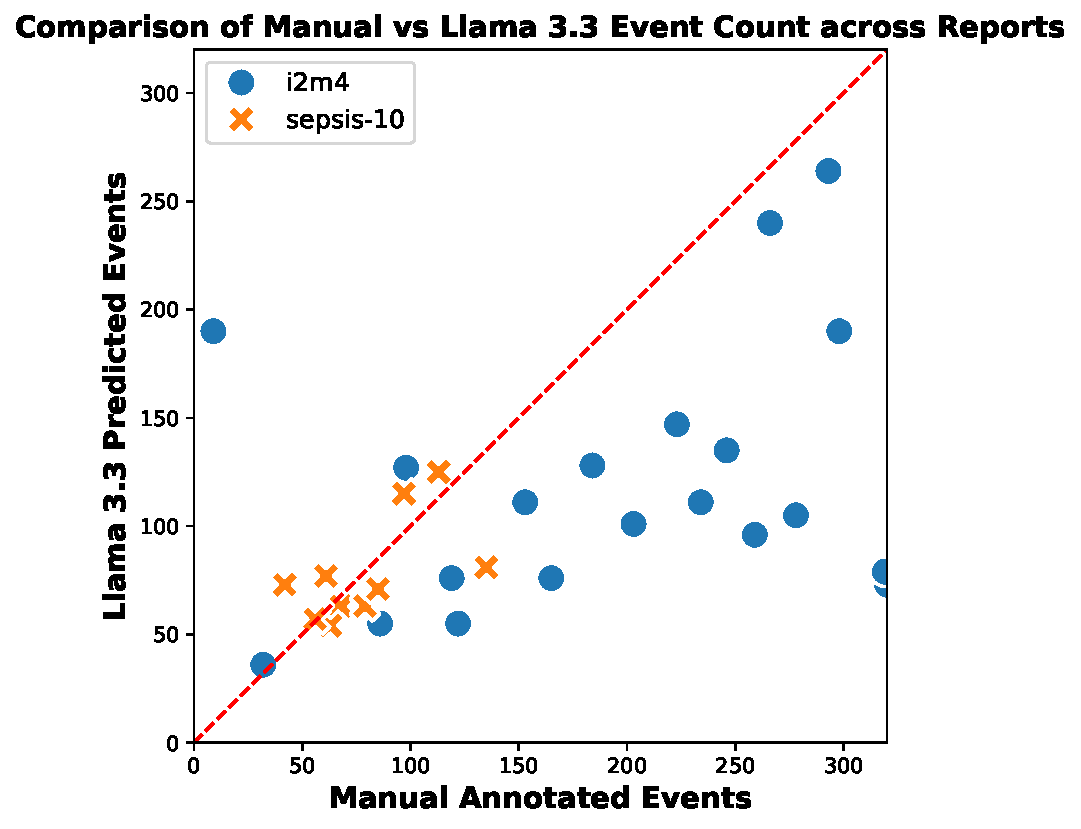
\includegraphics[width=0.7\linewidth]{Appendices/appendix-ch06/images/figures/manual_vs_l33_event_count.pdf}
    % \end{minipage}
    % \hfill
    
    

\end{ChSixFloatBody}
\caption{Comparison of Manual Annotation Clinical Event Counts and Llama 3.3 Model Predicted Event Counts: Scatter plot illustrating the variability between manual annotations and Llama 3.3 predictions across reports in two datasets, i2m4 (blue circles) and \texttt{sepsis-10} (orange crosses). The red dashed line indicates the ideal one-to-one correspondence where the number of events per report matches exactly between manual annotations and model predictions.}\ChSixFloatLabel{ch06:fig:manual_vs_l33_event_count}
\end{figure}



% !TeX root = ../../../main.tex
\begin{table}[htbp]
\caption{Proportion of reports where Llama 3.3 over- or under-identified clinical events compared to manual annotations. i2m4 shows a strong bias toward under-identification, whereas \texttt{sepsis-10} has a more balanced distribution.}\ChSixFloatLabel{ch06:tab:event_identification_bias}
\ChSixTableBodyStart
\begin{ChSixFloatBody}

\setlength{\tabcolsep}{4pt}
\centering
\begin{tabular}{|l|c|c|}
\hline
\textbf{Dataset} & \makecell{\textbf{\% Reports} \\ \textbf{Over-Identified}} & \makecell{\textbf{\% Reports} \\ \textbf{Under-Identified}} \\ \hline
\textbf{i2m4}    & 15\%                                & 85\%                                 \\ \hline
\textbf{\texttt{sepsis-10}} & 50\%                              & 50\%                                 \\ \hline
\end{tabular}



\end{ChSixFloatBody}
\end{table}


\ChSixParagraph{Dataset Structure Differences.}
The differences in dataset structure between i2m4 and \texttt{sepsis-10} are also evident in the length of clinical events.
As shown in Table~\ref{ch06:tab:character_length}, the manually annotated clinical events in i2m4 are significantly shorter, averaging $10\pm7$ characters, compared to $28\pm16$ characters in \texttt{sepsis-10}. 
This reflects the structured nature of i2m4 reports, which often include tables with abbreviations (e.g., ``K'' for Potassium, ``Na'' for Sodium). 
In contrast, \texttt{sepsis-10} reports are written in free text and provide full terms and descriptions, avoiding the abbreviation issue entirely. 
The absence of abbreviations in \texttt{sepsis-10} reduces variability in event representation and ensures greater alignment between manual annotations and Llama 3.3 predictions.


% !TeX root = ../../../main.tex
\begin{table}[htbp]
\caption{Average length of clinical events in characters for both datasets. Manual annotations in i2m4 are significantly shorter due to frequent abbreviations and structured text from MIMIC tables, while Llama 3.3 generates events of comparable length across datasets.}\ChSixFloatLabel{ch06:tab:character_length}
\ChSixTableBodyStart
\begin{ChSixFloatBody}

\centering
\begin{tabular}{|l|c|c|}
\hline
\textbf{Dataset} & \textbf{Manual Annotator} & \textbf{Llama 3.3} \\ \hline
\textbf{i2m4}    & $10\pm7 $                              & $17\pm14$                        \\ \hline
\textbf{\texttt{sepsis-10}} & $28\pm16$                            & $21\pm13$                        \\ \hline
\end{tabular}



\end{ChSixFloatBody}
\end{table}


Llama 3.3-generated clinical events are of similar length across datasets, with averages of $17\pm14$ characters for i2m4 and $21\pm13$ characters for \texttt{sepsis-10}. 
This consistency suggests that Llama 3.3 applies similar generative behavior across datasets, often producing expanded forms of abbreviations in i2m4. 
While this generative behavior mitigates variability in Llama 3.3 outputs, it creates a mismatch with the shorter, more concise manual annotations in i2m4. 
This mismatch can then contribute to higher cosine distances between embeddings, lowering the event match rate for i2m4.

\ChSixParagraph{Event Match Rate Insights.}
The event match rate, calculated as the proportion of manual clinical events correctly matched by Llama 3.3 predictions based on the sentence transformer embedding cosine distance threshold of 0.1, is significantly lower for i2m4 ($0.404$) than for \texttt{sepsis-10} ($0.753$). 
It should be noted that over-identification of clinical events by Llama 3.3 does not impact this metric, as in calculating the event match rate, we only consider events identified by the manual annotators. 
The observed difference can be attributed to two main factors:

\begin{itemize}
    \item Under-Identification Bias in i2m4: 
    When we adjust for under-identification by excluding manual clinical events for which Llama 3.3 did not identify a counterpart, the average match rate for i2m4 increases from $0.404$ to $0.752$, aligning more closely with \texttt{sepsis-10}'s match rate that increased from $0.753$ to $0.857$. 
    Figure~\ref{ch06:fig:match_rate_distributions} illustrates the match rate distributions across reports before and after the adjustment, highlighting the lower and more variable match rates in i2m4 compared to \texttt{sepsis-10}.
    This demonstrates that under-identification is the primary driver of the lower match rate in i2m4. 
    \item Dataset Structure Differences: 
    The structured nature of i2m4 reports introduces variability in the manual annotations due to the frequent use of abbreviations and table-like formats. 
    In contrast, the free-text nature of \texttt{sepsis-10} ensures more consistent and complete representations of clinical events. 
    While Llama 3.3 generates events of similar length across datasets, the expanded text spans of the abbreviations it generates in i2m4 exacerbate the mismatch with the manual annotations, leading to higher cosine distances and a lower event match rate.
\end{itemize}


% !TeX root = ../../../main.tex
\begin{figure}[htbp]
\begin{ChSixFloatBody}

\scriptsize
% \scriptsize
    % \begin{minipage}[t]{\columnwidth}
    \centering
    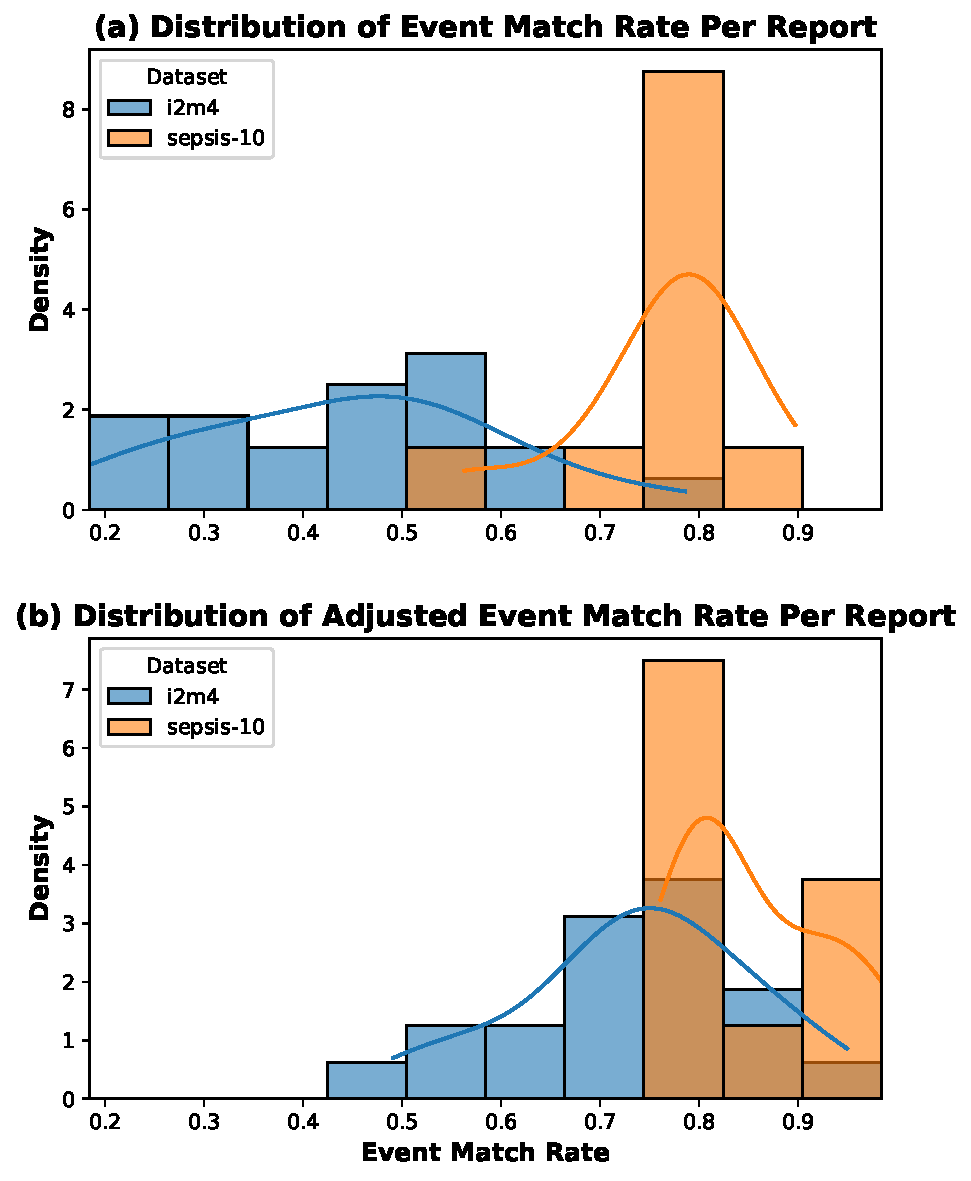
\includegraphics[width=0.7\linewidth]{Appendices/appendix-ch06/images/figures/match_rate_distributions.pdf}
    % \end{minipage}
    % \hfill
    
    

\end{ChSixFloatBody}
\caption{Distributions of Event Match Rates Across Reports Before and After Adjustment: 
    (a) Unadjusted Match Rate: Histogram and density plots of event match rates between manual annotations and Llama 3.3 predictions for reports in i2m4 (blue) and \texttt{sepsis-10} (orange). 
    The lower and more variable match rates in i2m4 highlight the impact of under-identification bias. 
    (b) Adjusted Match Rate: Histogram and density plots showing event match rates after excluding manual clinical events without Llama 3.3 counterparts. 
    The adjustment improves the match rates in i2m4, demonstrating that under-identification is the primary cause of its lower initial match rates compared to \texttt{sepsis-10}.}\ChSixFloatLabel{ch06:fig:match_rate_distributions}
\end{figure}


These findings demonstrate that the lower event match rate for i2m4 is at least partially driven by a systematic under-identification of clinical events by Llama 3.3 in this dataset, compounded by structural differences of reports in i2m4 versus \texttt{sepsis-10}. 

\subsubsection{Error Analysis of Temporal Predictions}
Across all models, i2m4 exhibits a lower concordance index (c-index) compared to \texttt{sepsis-10}. 
To better understand this discrepancy, we closely examine the performance of Llama 3.3, which shows similar trends in event ordering inconsistencies and a concordance-index drop from 0.93 to 0.75.

In i2m4, we observe higher variance in predicted event timestamps, with some extreme deviations from clinician annotations. To quantify the impact of these outliers, we apply an outlier filtering approach based on the interquartile range ($IQR$). 
The $IQR$ represents the middle 50\% of time differences, defined as the range between the first quartile ($Q1$, $25^{th}$ percentile) and the third quartile ($Q3$, $75^{th}$ percentile). 
Predictions falling outside $Q1 - 1.5 \times IQR$ or $Q3 + 1.5 \times IQR$ are removed, ensuring that event ordering is evaluated on a more stable subset of predictions.


% !TeX root = ../../../main.tex
\begin{figure}[htbp]
\begin{ChSixFloatBody}

\scriptsize
% \scriptsize
    % \begin{minipage}[t]{\columnwidth}
    \centering
    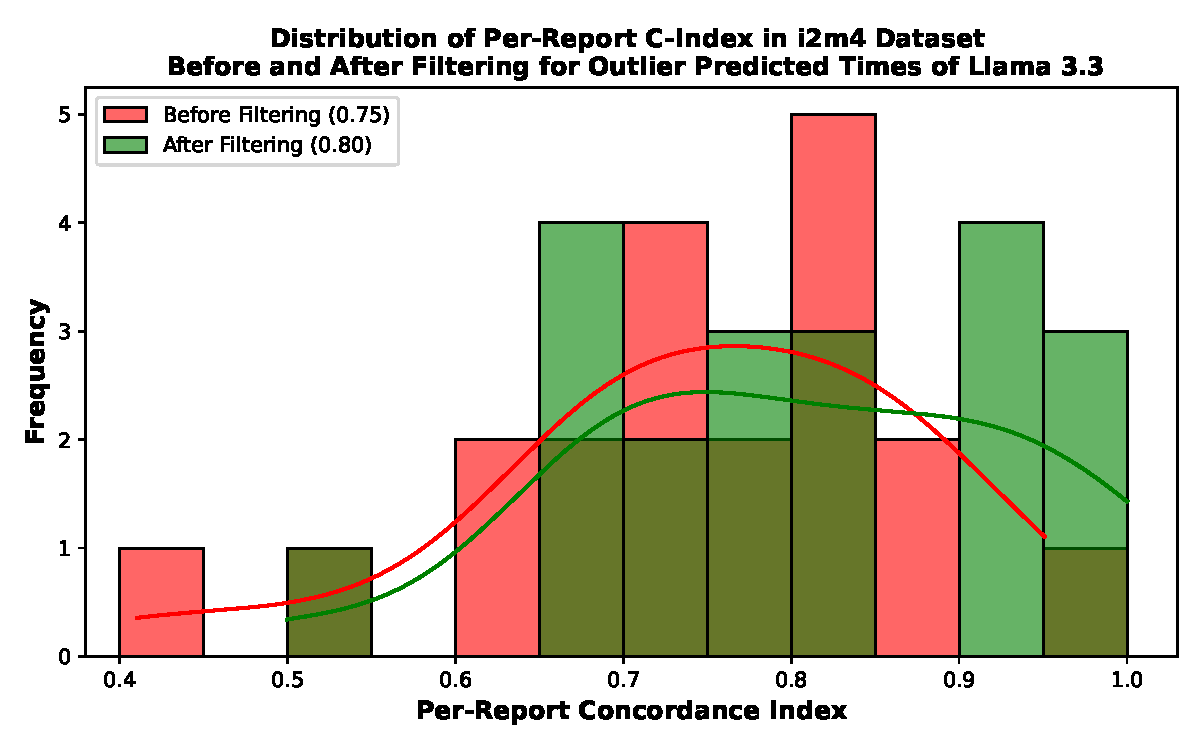
\includegraphics[width=0.7\linewidth]{Appendices/appendix-ch06/images/figures/cindex_outlier_filtering_l33.pdf}
    % \end{minipage}
    % \hfill
    
    

\end{ChSixFloatBody}
\caption{Effect of Outlier Filtering on c-index in i2m4. Distribution of per-report c-index before and after removing extreme time mispredictions using the interquartile range (IQR). Filtering improves the average c-index by reducing the impact of large temporal deviations.}\ChSixFloatLabel{ch06:fig:cindex_outlier_filtering_l33}
\end{figure}


After filtering, the average c-index for i2m4 improves from 0.75 to 0.80, suggesting that extreme time mispredictions were an important factor in lowering event ranking consistency. 
The shift in per-report c-index distribution after filtering further supports this observation as shown in Figure~\ref{ch06:fig:cindex_outlier_filtering_l33}. 
However, despite this improvement, i2m4’s c-index remains lower than \texttt{sepsis-10}, indicating that additional challenges, such as increased annotation complexity or structural differences in event distributions mentioned in the previous section, contribute to its overall lower performance. 

\subsubsection{Clinical Event Type Categorization Process}
\ChSixParagraph{Event Type Category Generation.}
To systematically categorize clinical events identified in case reports from two datasets, \texttt{sepsis-10} and i2m4, we employed a two-step methodology. 
The goal was to classify extracted clinical events into a predefined set of event type categories to use for further analysis of our results. 
Given i2m4's data protection provisions only allowed for local analysis, we used \texttt{sepsis-10} to determine the event type categories, as it was derived from PubMed Open Access case reports.

In the first step, event type categories were generated using a language model. 
Since the appropriate categories were not known a priori, we utilized OpenAI's o3-mini, to analyze all manually annotated clinical events from the \texttt{sepsis-10} dataset and derive six distinct event type categories. 
The model was prompted to examine the extracted events and construct a comprehensive yet non-overlapping set of categories that could effectively organize clinical events within the dataset. 
The full prompt used for this categorization process is as follows:

\begin{tcolorbox}[breakable,
  colback=yellow!10,
  colframe=orange!80!black,
  title=Event Type Category Generation Prompt,
  boxrule=2pt
]
\footnotesize
\setlength{\parskip}{1pt}
You are a physician and a machine learning scientist specializing in clinical event extraction. 

Your goal is to categorize extracted clinical events into exactly six distinct and mutually exclusive event categories to ensure clarity and consistency.

Constraints:
Each clinical event must belong to exactly one category.
The categories must be coarse enough to prevent ambiguity.
The sixth category is reserved for ``Other or Unknown.'' The first five categories should comprehensively cover the key types of clinical events.
The categories must be mutually exclusive, meaning an event should unambiguously fit into only one category.

Task:
Identify six well-defined, non-overlapping event categories that best classify the extracted clinical events.
Format the output as a comma-separated table with two columns:
Event Type Category: The name of the category.
Category Number: An integer from 0 to 5, with ``Other or Unknown'' always assigned to 5.

[Category Name], 0

[Category Name], 1

[Category Name], 2

[Category Name], 3

[Category Name], 4

Other or Unknown, 5

Now, based on the extracted clinical events below, generate six non-overlapping event categories and format the output as specified:

...all \texttt{sepsis-40} manual annotated clinical events...

\textless \textbackslash end prefix\textgreater
\end{tcolorbox}

The resulting six event type categories, along with their assigned numeric labels, were:

\begin{itemize}
    \item \textbf{Patient Background and Medical History (0)} -- Events describing patient demographics, prior medical conditions, risk factors, and relevant history before the clinical presentation.
    \item \textbf{Clinical Presentation and Examination Findings (1)} -- Events capturing the patient's initial symptoms, subjective complaints, and observable clinical signs from physical examination.
    \item \textbf{Diagnostic Testing and Results (2)} -- Events related to diagnostic investigations, including laboratory tests, imaging studies, and other diagnostic assessments, along with their results.
    \item \textbf{Clinical Management and Interventions (3)} -- Events detailing treatments and medical interventions, including pharmacological therapies, surgical procedures, and other clinical management strategies.
    \item \textbf{Clinical Course, Outcomes, and Follow-up (4)} -- Events describing the progression of the condition, response to treatment, complications, recovery, prognosis, and post-treatment follow-up.
    \item \textbf{Other or Unknown (5)} -- Events that do not clearly fit into the defined categories or contain insufficient information to be classified.
\end{itemize}

\ChSixParagraph{Event Type Category Assignment.}
Once these categories were established, they were used to systematically classify each identified clinical event from both \texttt{sepsis-10} and i2m4. 
The classification was performed separately for clinical events identified through manual annotation and those identified using Llama 3.3. 
To maintain compliance with IRB regulations, all event classifications, including those for i2m4, were executed on a local machine to prevent data transfer to external servers.

For this classification step, we used Llama 3.3 to assign each extracted clinical event to one of the six predefined event type categories. 
The model was provided with a prompt that explicitly listed all event type categories and required it to assign each event to the most appropriate category. 
The classification was performed for both manually annotated events and events identified by Llama 3.3 across the \texttt{sepsis-10} and i2m4 datasets. 
The exact prompt used for this classification task is as follows (the green text includes the few-shot examples provided to the model):

\begin{tcolorbox}[breakable,
  colback=yellow!10,
  colframe=orange!80!black,
  title=Event Categorization Prompt,
  boxrule=2pt
]
\footnotesize
\setlength{\parskip}{1pt}
You are a medical professional. 

You are tasked with categorizing clinical events extracted from case reports.

Assign the following clinical event to one of these categories.

The categories are:

Patient Background and Medical History: 0,

Clinical Presentation and Examination Findings: 1,

Diagnostic Testing and Results: 2,

Clinical Management and Interventions: 3,

Clinical Course, Outcomes, and Follow‐up: 4,

Other or Unknown: 5
\\
The categories are defined as follows:

Patient Background and Medical History: (Includes demographic details, prior medical diagnoses, past surgical histories, medication use as part of chronic history, and other baseline background information.),

Clinical Presentation and Examination Findings: (Includes symptoms at presentation, physical exam findings---including vital signs, neurological scores that reflect exam observations---and other immediate clinical observations.),

Diagnostic Testing and Results: (Includes all imaging studies, laboratory tests, diagnostic procedures and their reported findings, and formal diagnostic conclusions reached via workup.),

Clinical Management and Interventions: (Includes all treatments, procedures, medications administered acutely, operations, supportive care measures, and decisions/interventions intended to alter the patient’s condition.),

Clinical Course, Outcomes, and Follow‐up: (Includes statements about change in clinical status, response to treatment, complications, transitions in care, recovery, discharge, and long‐term outcomes.),

Other or Unknown: (For events that do not clearly fit into any of the above five categories.)

\color{ChSixDarkTeal}
For example, here is a list of clinical event text and the corresponding category:

Examples:

``60-year-old female'' → 0

``history of atrial fibrillation'' → 0

``weighed 95 kg'' → 0

``Impaired consciousness'' → 1

``high-grade fever'' → 1

``persistently high-temperature spikes'' → 1

``Head CT'' → 2

``no hepatitis A'' → 2

``stage IV lymphoma'' → 2

``successfully treated with fidaxomicin'' → 3

``shifted to cefepime'' → 3

``intravenous immunoglobulins for 5 days'' → 3

``follow-up evaluations were recommended'' → 4

``transferred to a geriatric medicine unit'' → 4

``Discharge'' → 4

``he'' → 5

``confined, 5

``other symptoms'' → 5
\color{black}

Event: ``$\{\text{event}\_\text{text}\}$''

Respond with only the corresponding integer (0-5) from the list above.
You have to pick only one category for each event. 
If there is no clear category, choose the category 5 that corresponds to ``Other or Unknown'' category.
If there is more than one category, choose the category that you think is most relevant one.
Do NOT include any extra text in your response. Do NOT show your thought process.
Only provide the integer corresponding to the category and nothing else.

Format your response as:

Response: \textless integer \textgreater

\textless \textbackslash end prefix\textgreater
\end{tcolorbox}

\ChSixParagraph{Event Type Category Alignment and Match Rate Analysis.}  

To assess the consistency of event type categorization between the two annotators (manual annotator vs. Llama 3.3), we computed the event type category alignment rate for each dataset separately.  
This metric quantifies how often the manually annotated events and the Llama 3.3-extracted events---when determined to be aligned---are also assigned to the same event type category.  

For each case report in the dataset, clinical events extracted by the manual annotator were aligned with those extracted by Llama 3.3 using an iterative matching approach based on the cosine distance of their sentence-transformer embeddings.  
Aligned event pairs, which consist of one event from the manual annotator and one from Llama 3.3, were then categorized independently by Llama 3.3 into one of six predefined event type categories of the previous section.  

The event type category alignment rate was computed by determining, for each aligned event pair, whether both events were assigned to the same category.  
If both events in an aligned pair received the same category label, the event type alignment was considered successful.  
For each dataset, the event type alignment rate was first calculated per case report by dividing the number of successfully aligned event type pairs by the total number of aligned pairs in that case report.  
These per-case alignment rates were then averaged across all case reports in the dataset to obtain the final alignment rate.  
Table \ref{ch06:tab:event_category_alignment} reports the mean alignment rate along with the standard deviation for each dataset. 

The event type category alignment rate was higher for the i2m4 dataset ($0.71 \pm 0.05$) compared to the \texttt{sepsis-10} dataset ($0.56 \pm 0.05$).  
We hypothesize that this discrepancy is due to the absence of the ``Other or Unknown'' category in the \texttt{sepsis-10} dataset, which likely introduced ambiguity in category assignments.  
Specifically, since no events in \texttt{sepsis-10} were assigned to the ``Other or Unknown'' category, the model may have redistributed events that would have otherwise fallen into this category among the other five categories.  
This misalignment in categorization likely contributed to the lower agreement rate between the two annotators in the \texttt{sepsis-10} dataset.  


% !TeX root = ../../../main.tex
\begin{table}[htbp]
\caption{Mean event type category alignment rate between the manual annotator and Llama 3.3 for each dataset.  
The alignment rate is computed as the proportion of aligned event pairs that were assigned to the same event type category.  
The reported values represent the mean alignment rate across case reports, with standard deviation indicated.}\ChSixFloatLabel{ch06:tab:event_category_alignment}
\ChSixTableBodyStart
\begin{ChSixFloatBody}

\centering
\begin{tabular}{|l|c|}
\hline
\textbf{Dataset} & \textbf{Event Type Alignment} \\ \hline
\textbf{i2m4}    & $0.71\pm0.05 $                       \\ \hline
\textbf{\texttt{sepsis-40}} & $0.56\pm0.05$                      \\ \hline
\end{tabular}



\end{ChSixFloatBody}
\end{table}


To further investigate the impact of event type categorization on event match rates, we analyzed the match rate separately for each of the six predefined event categories within both datasets.  
Figure \ref{ch06:fig:event_match_rate_per_category} displays the mean match rate for each event category, with error bars representing the standard deviation across case reports.  
The dashed horizontal lines indicate the overall mean match rate for all event types within each dataset (as seen in Table~\ref{ch06:tab:results}), providing a point of reference for comparison.

From the figure, it is evident that the event match rates exhibit variability across categories but do not show significant deviations that would suggest one category consistently performs better or worse than the others.  
For instance, in both datasets, categories such as ``Diagnostic Testing and Results'' and ``Clinical Course, Outcomes, and Follow up'' tend to achieve higher match rates compared to others, though the differences are not substantial enough to be statistically significant.  
Similarly, the match rates for ``Clinical Management and Interventions'' and ``Patient Background and Medical History'' fall closer to the overall dataset mean, suggesting these categories are neither particularly challenging nor exceptionally easy for alignment.

A notable observation is the ``Other or Unknown'' category, which is entirely absent in the \texttt{sepsis-10} dataset.  
This absence introduces a unique challenge for categorization, as events that might have otherwise been assigned to this category are redistributed among the remaining categories.  
The i2m4 dataset, on the other hand, includes this category, and has a moderate event match rate for the event types in this category.  
This discrepancy could partially suggest that the style, structure, or format of the \texttt{sepsis-10} dataset differs from that of i2m4.  
The absence of the ``Other or Unknown'' category in \texttt{sepsis-10} could indicate a more standardized or narrowly focused structure, where fewer ambiguous or unclassifiable events are present, whereas i2m4 may include a broader range of events requiring such a fallback category.  
This difference in dataset characteristics could contribute to the observed variability in event match rates, as the annotation and alignment processes are inherently influenced by the dataset's structure and complexity.  


% !TeX root = ../../../main.tex
\begin{figure}[htbp]
\begin{ChSixFloatBody}

\scriptsize
% \scriptsize
    % \begin{minipage}[t]{\columnwidth}
    \centering
    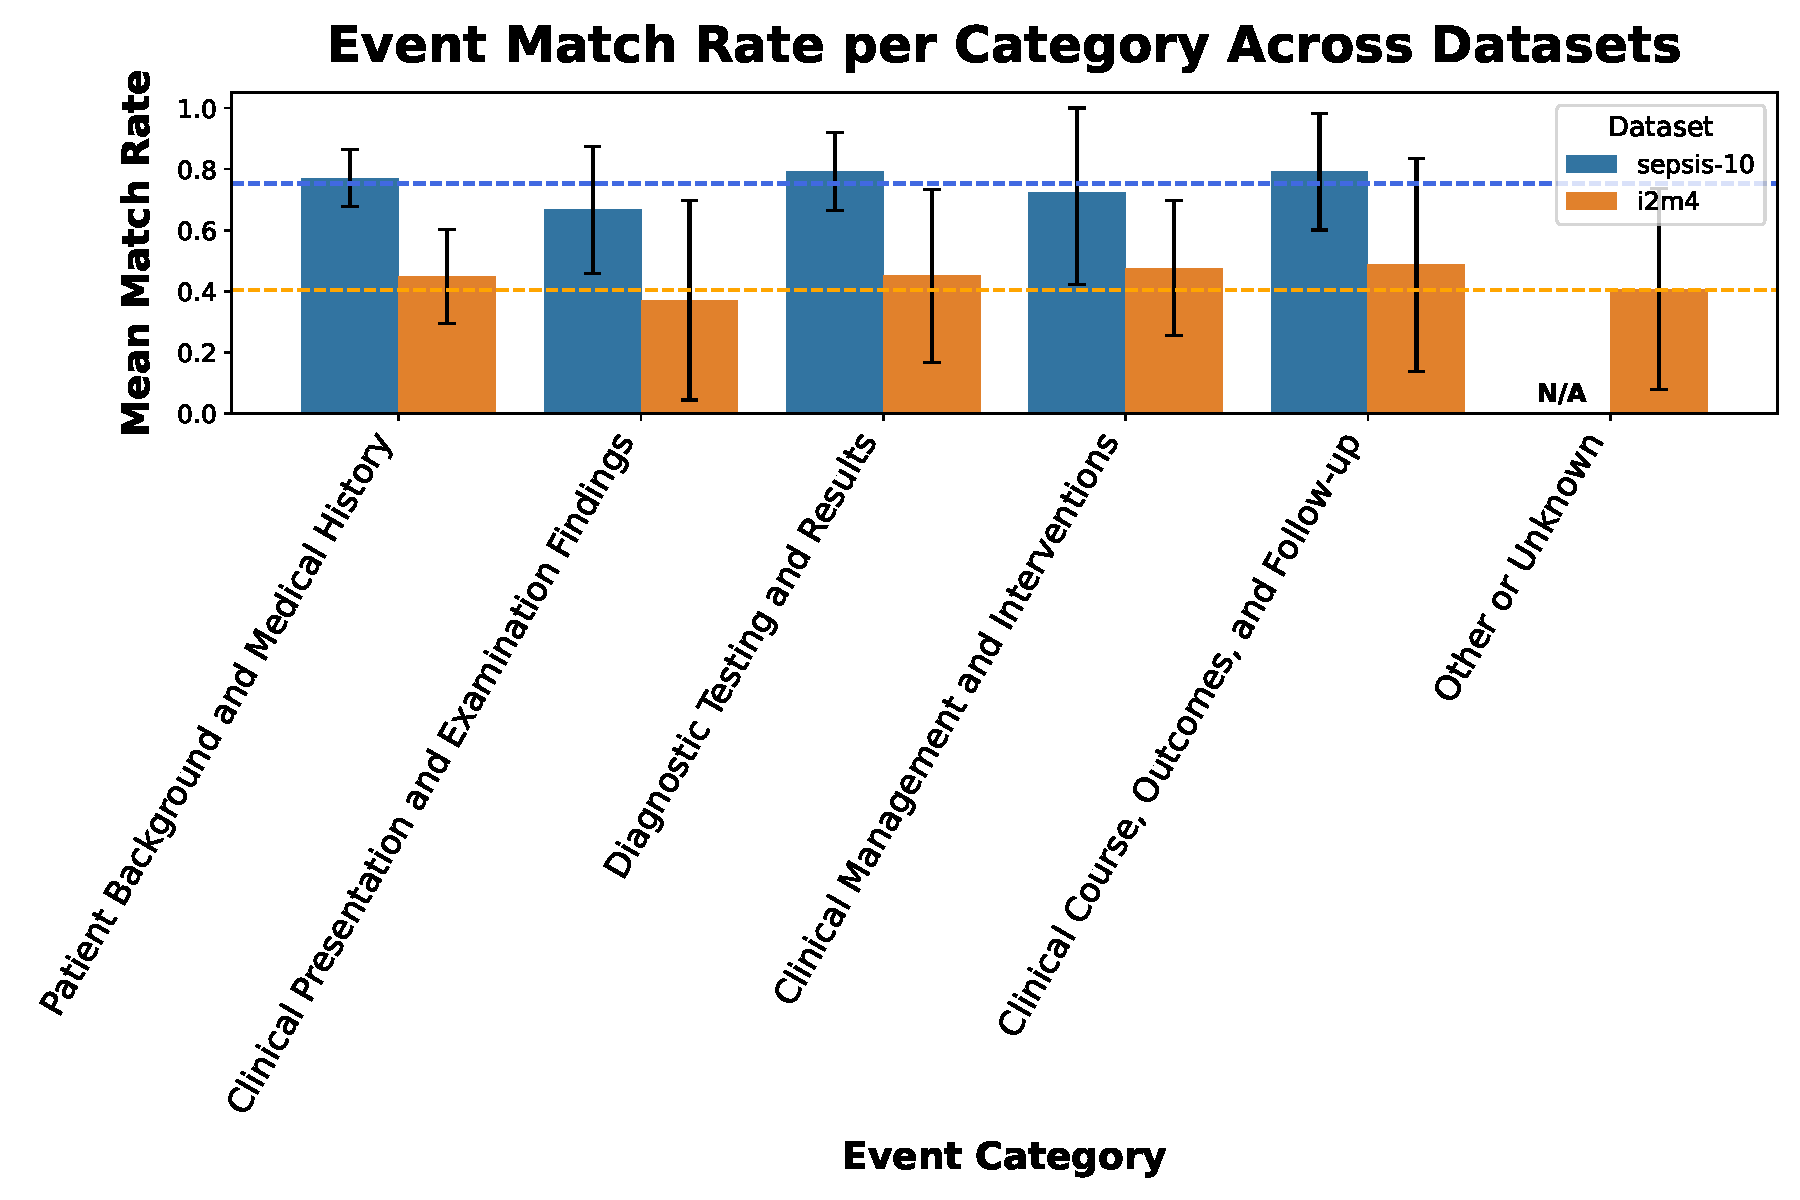
\includegraphics[width=0.9\linewidth]{Appendices/appendix-ch06/images/figures/event_match_rate_per_category.pdf}
    % \end{minipage}
    % \hfill
    
    

\end{ChSixFloatBody}
\caption{Mean event match rate across predefined event type categories for the i2m4 and \texttt{sepsis-10} datasets.  
    Bars represent the mean match rate for each event type category, calculated as the proportion of aligned event pairs (between the manual annotator and Llama 3.3) with cosine distance less than the matching threshold.  
    Error bars indicate the standard deviation of match rates across case reports.  
    The dashed lines represent the overall mean match rates for each dataset across all categories (From Table~\ref{ch06:tab:results}: \textcolor{blue}{\texttt{sepsis-10}}: 0.753 and \textcolor{orange}{i2m4}: 0.404)
    The ``Other or Unknown'' category is absent in \texttt{sepsis-10}, resulting in no match rate for this category in that dataset.}\ChSixFloatLabel{ch06:fig:event_match_rate_per_category}
\end{figure}


Overall, the analysis suggests that event match rates are relatively stable across event categories within each dataset.  
The differences in overall match rates between i2m4 and \texttt{sepsis-10} (and hence \texttt{sepsis-40}) are therefore more likely attributable to dataset-specific characteristics and under-identification bias that was explained in the previous section.
Future work could explore more granular metrics, such as examining the semantic content of events within each category, to better understand the nuances of these event match rate discrepancies. 

